\documentclass[12pt]{article}
\usepackage{geometry}                % See geometry.pdf to learn the layout options. There are lots.
\geometry{letterpaper}                   % ... or a4paper or a5paper or ... 
%\geometry{landscape}                % Activate for for rotated page geometry
\usepackage[parfill]{parskip}    % Activate to begin paragraphs with an empty line rather than an indent
\usepackage{daves,fancyhdr,natbib,graphicx,dcolumn,amsmath,lastpage,url}
\usepackage{amsmath,amssymb,epstopdf,longtable}
\usepackage{paralist}  % need to properly formulate standard answer blocks
\usepackage[final]{pdfpages}
\DeclareGraphicsRule{.tif}{png}{.png}{`convert #1 `dirname #1`/`basename #1 .tif`.png}
\pagestyle{fancy}
\lhead{CE 3305 Fluid Mechanics; Exercise Set 13}
\rhead{Name:\_\_\_\_\_\_\_\_\_\_\_\_\_\_\_\_\_\_\_\_\_\_\_\_\_\_\_\_\_\_\_\_\_\_}
\lfoot{REVISION A}
\cfoot{}
\rfoot{Page \thepage\ of \pageref{LastPage}}
\renewcommand\headrulewidth{0pt}
%%%%%%%%%%%%%%%%%%%%%%%%%%%%%%%%%%%%
\begin{document}
%%%%%%%%%%%%%%%%%%%%%%%%%%%%%%%%%%%
\begingroup
\begin{center}
{\textbf{{ CE 3305 Engineering Fluid Mechanics} \\ Exercise Set 13 \\ Summer 2018 -- GERMANY} }
\end{center}
\endgroup
\begingroup
~\newline
\textbf{Purpose} :  Momentum balance \\
\textbf{Assessment Criteria} : Completion, plausible solutions, use \textbf{R} as a calculator. \\~\\
\textbf{Exercises}

\begin{enumerate}
\item (Problem 6.7 pg 238)  Figure \ref{fig:JetBalloon} is a balloon rocket held in place by a force $F$.  
The nozzle is a 0.8 $cm$ diameter tube, and an air jet exits the nozzle with a speed of 45 $m/s$ and a density of 1.2 $kg/m^3$.  Find the force $F$ needed to hold the balloon stationary.
\begin{figure}[h!] %  figure placement: here, top, bottom, or page
   \centering
   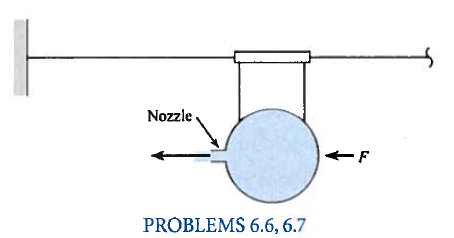
\includegraphics[width=3in]{JetBalloon.jpg} 
   \caption{Balloon rocket}
   \label{fig:JetBalloon}
\end{figure}



\item (Problem 6.16 pg 239) 
Figure \ref{fig:JetBoat} is a schematic of a boat held stationary by a cable attached to a pier.  
A firehose directs a jet of 5 $^oC$ water at a speed of $V = 50 m/s$.  
The allowable load on the cable is 5 $kN$.
Determine:
\begin{enumerate}
\item The mass flow rate of the water jet.
\item The diameter of the water jet.
\end{enumerate}

\begin{figure}[h!] %  figure placement: here, top, bottom, or page
   \centering
   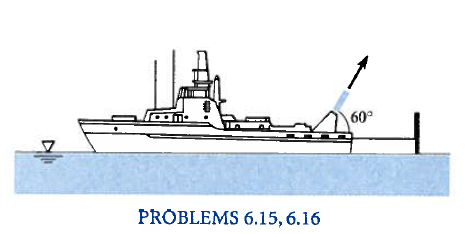
\includegraphics[width=3in]{JetBoat.jpg} 
   \caption{Fire boat restrained by a cable}
   \label{fig:JetBoat}
\end{figure}
\clearpage

\item (Problem 6.63 pg 246) Figure \ref{fig:PipeBend} is a schematic of an elbow fitting in a pipe system.  The gage pressure throughout the horizontal 90$^o$ bend (the elbow lies in the horizontal plane -- the figure is a plan view of the bend) is 300 $kPa$.  
If the pipe diameter is 1 $m$ and the water (at 10 $^oC$) flow rate is 10 $m^3/s$, what $x-$component of force must be applied to the bend to hold in in place against the water action.

\begin{figure}[h!] %  figure placement: here, top, bottom, or page
   \centering
   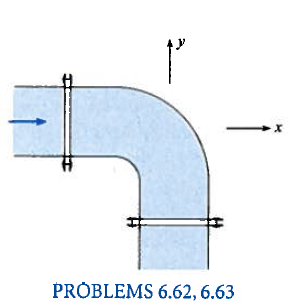
\includegraphics[width=2in]{PipeBend.jpg} 
   \caption{Elbow fitting on a pipe line.}
   \label{fig:PipeBend}
\end{figure}


\end{enumerate}
\end{document}  